%----------------------------------------------------------------------------------------------------------------------------------------------------------%
\chapter{Theoretical context}
%----------------------------------------------------------------------------------------------------------------------------------------------------------%
\epigraph{Each source that I read, I would look through the bibliography and the footnotes, and use that as a map for the next thing I would read.}{\textit{Alexander Chee}}
%----------------------------------------------------------------------------------------------------------------------------------------------------------%
\section{Bacteria and bacterial infections}
\paragraph{Bacteria} are prokaryotic organisms, generally single-celled, which are part of the Monera kingdom. Their sizes range from between 30\textmu m and 100\textmu m and are ubiquitous\footnote{Ubiquitous: found everywhere} organisms. This form of life is believed to be the first one to have ever appeared on Earth, as well as the one responsible for the oxygen-rich atmosphere the Earth currently has. Some species are hard to culture in a laboratory environment, but generally, those that can be cultured in a controlled environment are grown in agar plates\cite{murrayMicrobiologiaMedica2013}. \newline
\paragraph{Pathogenic bacteria} are bacteria that have the ability to cause disease\footnote{A disease is a particular abnormal condition that negatively affects the structure or function of all or part of an organism, and that is not immediately due to any external injury\cite{DorlandsMedicalDictionary2010}.} These are not the most common type of bacteria, as the majority of them are either harmless or beneficial to the human body through symbiosis, such as the bacteria that help with digestion in the stomach\cite{murrayMicrobiologiaMedica2013}.
%----------------------------------------------------------------------------------------------------------------------------------------------------------%
\section{The enemy: \emph{Staphylococcus aureus}}
\paragraph{}\emph{Staphylococcus aureus} (also known as Staph) is a GRAM-positive bacterium, usually not pathogenic. It can, in some cases, cause extremely dangerous infections. Some of its distinctive characteristics include a very thick glycopeptide wall, which allows it to withstand extreme temperatures and osmotic pressures, rendering most classic methods of food conservation\footnote{Cooking, smoking, freezing, salting...} useless against it; a protein A capsid, which binds to most eukaryote cells; as well as thermoresistant enterotoxins. It's a bacterium that can resist many environments, and can found on human skin, mucotic surfaces, as well as in certain foods such as ham, eggs, and poultry\cite{nutritionBAMChapter122020}.\newpage
\begin{wrapfigure}{r}{0.5\textwidth}\begin{center}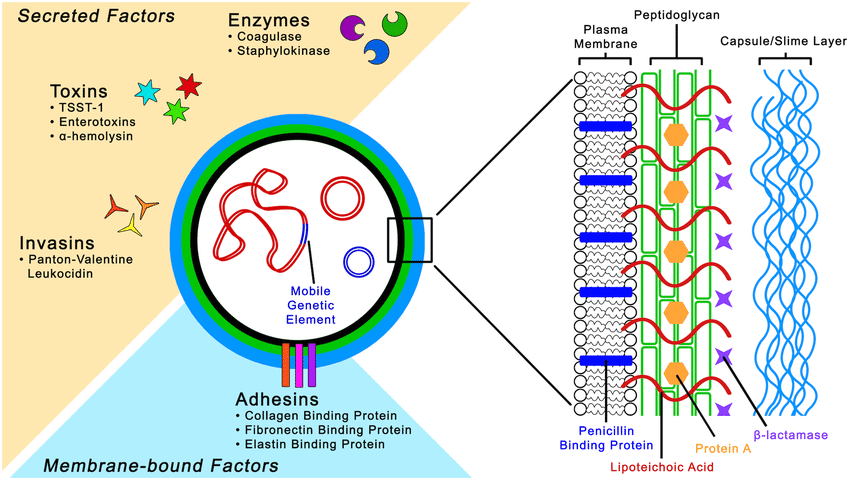
\includegraphics[width=0.48\textwidth]{staph_parts.png}\end{center}\caption{Parts of \emph{Staphylococcus aureus}\cite{kongCommunityAssociatedMethicillinResistantStaphylococcus2016}.}\end{wrapfigure}
\paragraph{}Staphylococcus aureus has three main parts to its virulence: its cell wall, its membrane-bound factors and its secreted factors. Staph's cell wall is made up of three parts. From the inside out they are: a plasma membrane, a peptidoglycan layer and a capsule\cite{kongCommunityAssociatedMethicillinResistantStaphylococcus2016}.
The membrane includes a semipermeable lipid bi-layer, which regulates the transport of materials entering and exiting the cell. Integrated inside it are a type of integral protein called penicillin-binding protein (PBP), along with proteins dedicated to powered transport. We are only interested in PBPs. Even though the name
 implies PBPs are only sensible to penicillin, the name actually came to be this way because of their discovery. These proteins are sensitive to the \textbeta-lactam groups in antibiotics. Variations in them may lead to antibiotic-resistant strains, such as MRSA (\emph{Methicillin-Resistant \emph{Staphylococcus aureus}}), result of a mutation in this protein called PBPA2\cite{kongTargetingStaphylococcusAureus2016}. \newline
\emph{Staphylococcus aureus}, like all other members of the \emph{Staphylococcus} family, has a very thick peptidoglycan layer. This grants them protection from extreme temperatures and high osmotic pressures. Since little to no other bacteria can survive in the conditions that Staph can, it starts reproducing without the limit that would be imposed by having other bacteria competing for the same resources\cite{clareticomaResistenciaAntibioticaPoblacions2004}.
%----------------------------------------------------------------------------------------------------------------------------------------------------------%
\section{The enemy's attacks}
\paragraph{}\emph{Staphylococcus aureus} is a species that can cause a handful of different diseases, ranging from, most frequently, skin and respiratory tract infections to infective endocarditis, toxic shock syndrome or osteomyelitis\cite{cheungPathogenicityVirulenceStaphylococcus2021}. Several variations of this pathogen exist, with increasing levels of antibiotic resistance: MSSA (\emph{Methicillin-Sensitive Staphylococcus aureus}), having no resistance; MRSA (\emph{Methicillin-Resistant Staphylococcus aureus}); and VRSA (\emph{Vancomycin-Resistant Staphylococcus aureus}), the   latter for which no antibiotic concoction that can eradicate the infection is known, and the patients have to use experimental treatments. VISA (\emph{Vancomycin-intermediate Staphylococcus aureus}) is a variation that has medium resistance to vancomycin, being an intermediate step between MRSA and VRSA. Studies have discovered that this genetic factor has been developed by different lineages separately, indicating that there is not a common ancestor of MRSA strains\cite{zhouReviewNanosystemsEffective2018}.
\paragraph{}\emph{Staphylococcus aureus} contains an important quantity of \textbf{toxins}, compounds that grant \emph{Staph} most of its pathogenicity. Many of its virulence factors can be described as such. Toxins are usually defined as poisonous substances, which, in our case, means that they have the capacity to mess with the host body directly, without need of a mediating entity. Staph has several kinds of toxin in its arsenal: membrane-damaging toxins (which can be receptor-mediated or not), receptor-interfering toxins (which do not damage the membrane), enzymes, and pathway blockers\cite{kongTargetingStaphylococcusAureus2016}.\newline
%----------------------------------------------------------------------------------------------------------------------------------------------------------%
\section{Our weapons}
\paragraph{} The tools we have at our disposal to fight off this infection fall into two main categories: chemical factors and biological factors.
\paragraph{} The chemical factors are drugs, and they depend both in quantity and type on the variation a particular case falls in. It is \textbf{extremely important} to find out the level of antibiotic resistance that a specific infection has before administering any antibiotic, as this treatment course will cause side effects such as killing gut bacteria, diminishing defence system capabilities, and increasing the possibility to develop yet more resistant infections. Generally, a large-spectrum antibiotic has an adequate risk-to-benefits ratio of causing the previously mentioned side effects, so they may be used before switching to a more specific (and in some cases even more violent) treatment.
\paragraph{}\begin{wrapfigure}{r}{0.35\textwidth}\begin{center}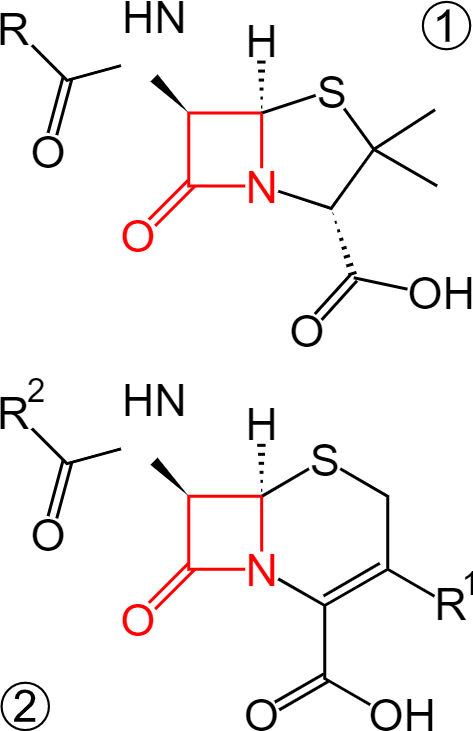
\includegraphics[width=0.30\textwidth]{assets/beta-lactam.png}\end{center}\caption{Organic chemistry structure of penicillin (top) and cephalosporin (bottom). The \textbeta-lactam ring is indicated in red. Source: \cite{fvasconcellosSkeletalFormulaeBasic}}\vspace{-0.30\linewidth}\end{wrapfigure}Starting with the treatment to the least resistant strains of \emph{Staphylococcus aureus}, a \textbeta-lactam antibiotic (such as methicillin, oxacillin, cloxacillin and penicillin) is the weapon of choice to fight against an MSSA infection. This is because this specific chemical part (just a \textbeta-lactam ring does nothing by itself) has the ability to inhibit cell wall biosynthesis on the bacterial intruder's body. But once the \textbeta-lactam ring is cut by an enzyme secreted by the bacteria itself, this type of antibiotic suddenly loses effect against them.
\paragraph{}That's where vancomycin comes in. It is a type of glycopeptide antibiotic, just like \textbeta-lactam, and works by blocking the construction of a cell wall, as all of its type do.
\begin{wrapfigure}{l}{0.35\textwidth}\begin{center}
\includegraphics[width=0.30\textwidth]{assets/vancomycin.png}\end{center}\caption{Organic chemistry structure of vancomycin. Source: \cite{bartvl71ChemicalStructureVancomycin}}\vspace{0.15\linewidth}\end{wrapfigure}This treatment is very invasive and only indicated for the treatment of extremely serious, life-threatening infections by Gram-positive bacteria that have shown to be unresponsive to other antibiotics.It can be taken as a pill or as an injectable fluid, the latter form proving to be much more effective than the former. This treatment is incompatible with aminoglycosides, a type of antibiotic that inhibits protein synthesis, as it can lead to nephrotoxicity and ototoxicity. Vancomycin can induce  internal bleeding, with petechial haemorrhages on the tongue and bruises on most of the body of the patient. Unfortunately, even with use of vancomycin, \emph{Staphylococcus aureus} can develop resistance. In this case, no other option than using a biological factor is left.
\newpage\paragraph{}The biological factor is a bacteriophage, called P68. It comes from the \emph{Caudovirales} order, which means that it is a bacteriophage with tail.  This treatment is still in testing, but it appears to be effective and lead to low adverse results. If possible, it would be preferable to use bacteriophage therapy (shortened to phage therapy) instead of going for antibiotics, as it can lead to less side effects than antibiotics, as it only attacks a specific bacterium. This means that the infection has to be pinpointed with extreme accuracy. The use of this treatment also negates the risk of bacteria developing antibiotic resistance. It is, however, unclear whether the bacteriophage could mutate into a dangerous strain. This therapy is in clinical research, and may be available soon.\cite{zhouReviewNanosystemsEffective2018}\cite{eskenaziCombinationPreadaptedBacteriophage2022}.
\newpage{}\begin{wrapfigure}{r}{0.35\textwidth}\begin{center}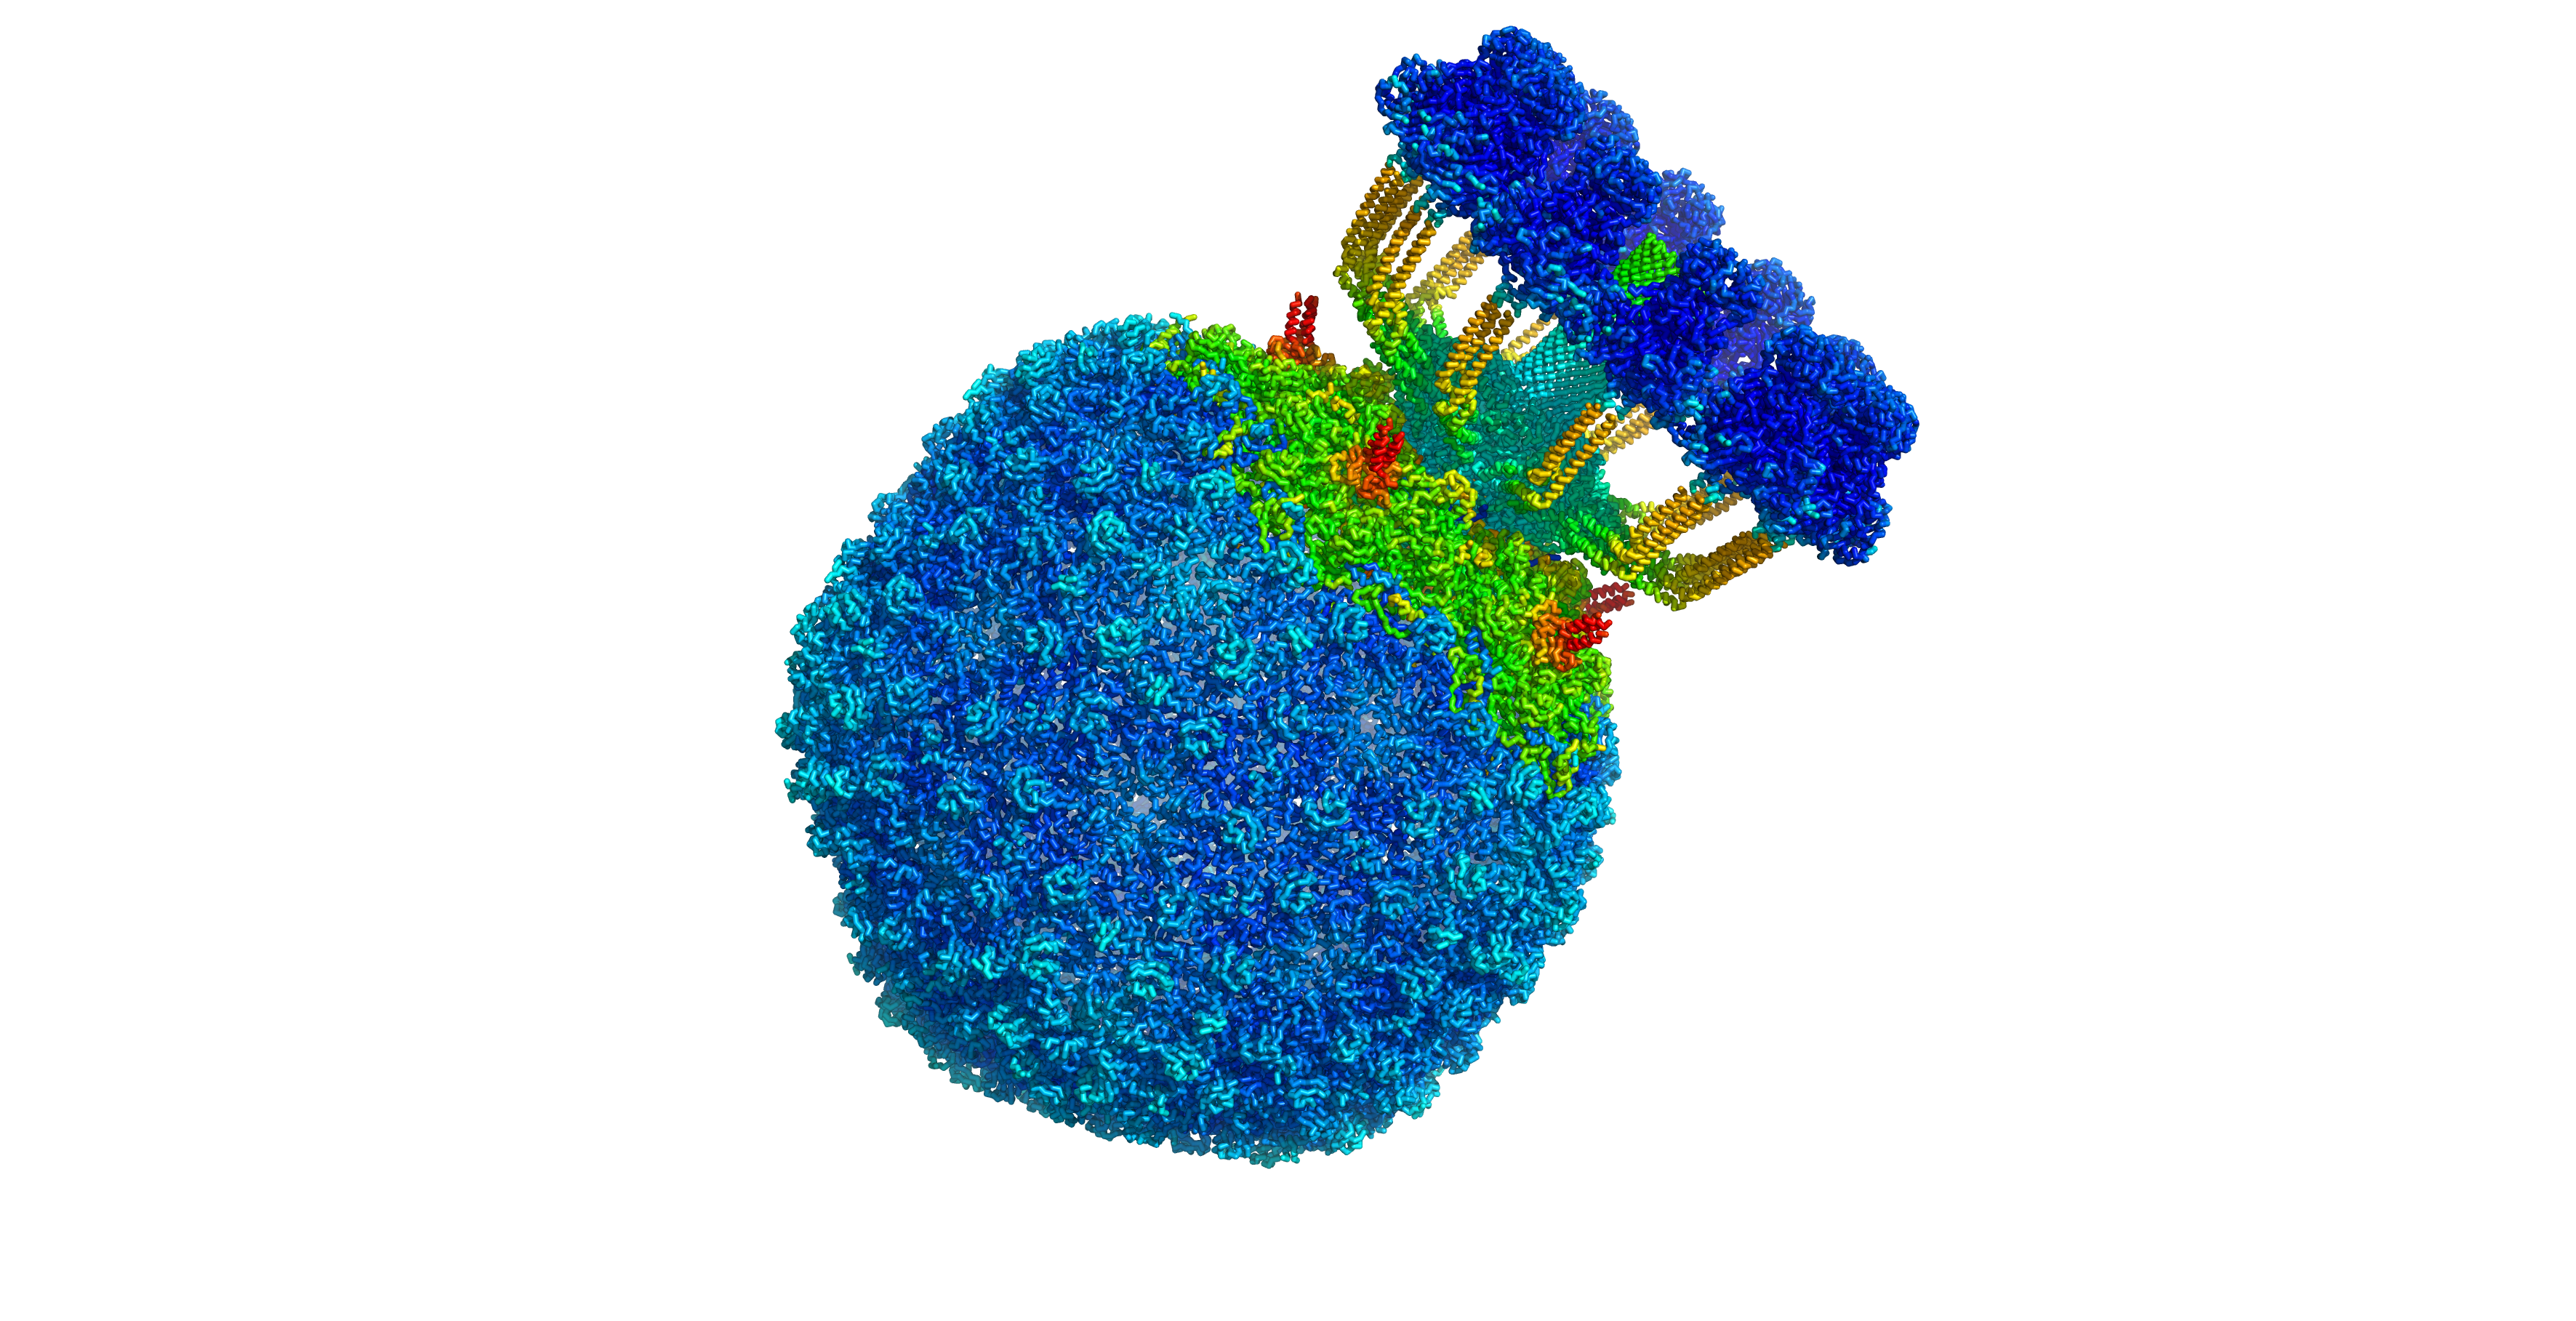
\includegraphics[width=0.30\textwidth]{assets/staph_side.png}\end{center}\caption{P68 structure. Source: own}\end{wrapfigure}Bacteriophages work in an interesting manner. They work by detecting one very specific bacteria, just like any other virus does with the type of cell they evolved for, then bind to it and inject their genetic material, which then in turn the bacteria considers as its own, inserts it into its own genetic sequence and starts producing the proteins the virus requires, but it doesn't eject them. Once the bacteria is full of phages, a special lytic compound is released which bursts the cell membrane in such a way that it resembles an explosion, but instead of heating up everything in a radius, spreads millions more of bacteriophages, which then bind to other bacteria and the cycle repeats until there's no more bacteria left. The fight from the bacteria point of view consists mostly on trying to outnumber and outreproduce the phages in order to have a chance of survival, even if minimal. There is no known bacteria that shows resistance to phages. That is probably because, unlike the chemical factors, phages can evolve and improve with each generation thanks to natural selection\cite{hrebikStructureGenomeEjection2019a}.
